\section{Introduction}
% \begin{frame}{Introduction}{Motivation}
%   \begin{figure}[!hbt]
%     \centering
%     \scalebox{.7}{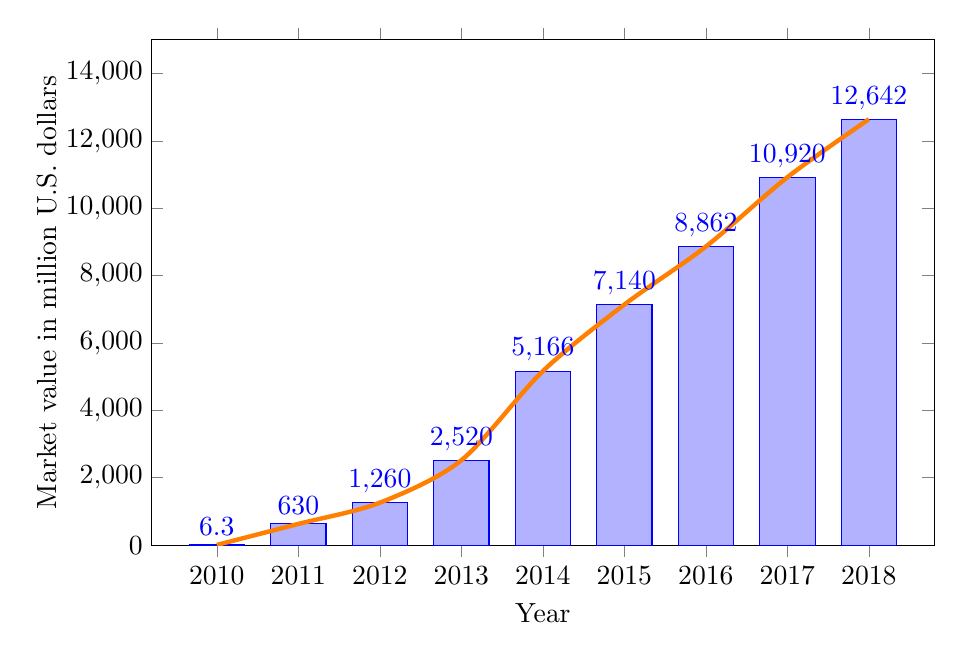
\begin{tikzpicture}
    \begin{axis}[
        height=8cm,
        width=0.95\textwidth,
        xlabel={Year},
        ylabel={Market value in million U.S. dollars},
        yticklabel style={align=right,inner sep=0pt,xshift=-0.3em},
        scaled y ticks = false,
        nodes near coords align={vertical},
        nodes near coords,
        xtick=data,
        symbolic x coords={2010, 2011, 2012, 2013, 2014, 2015, 2016, 2017, 2018},
        ymax=15000,
        ymin=0,
        ybar, 
        bar width=20pt
        ]
        \addplot coordinates {(2010, 6.3) (2011, 630) (2012, 1260) (2013, 2520) (2014, 5166) (2015, 7140) (2016, 8862) (2017, 10920) (2018, 12642)};
        \addplot [ultra thick,orange,line join=round,smooth, nodes near coords = ] coordinates {(2010, 6.3) (2011, 630) (2012, 1260) (2013, 2520) (2014, 5166) (2015, 7140) (2016, 8862) (2017, 10920) (2018, 12642)};
%        
    \end{axis}
\end{tikzpicture}}
%     \caption{Wearable trend. Data from Statista.}
%   \end{figure}
% \end{frame}

% \begin{frame}{Introduction}{Motivation}
%   \begin{figure}[!hbt]
%     \centering
%     \scalebox{.7}{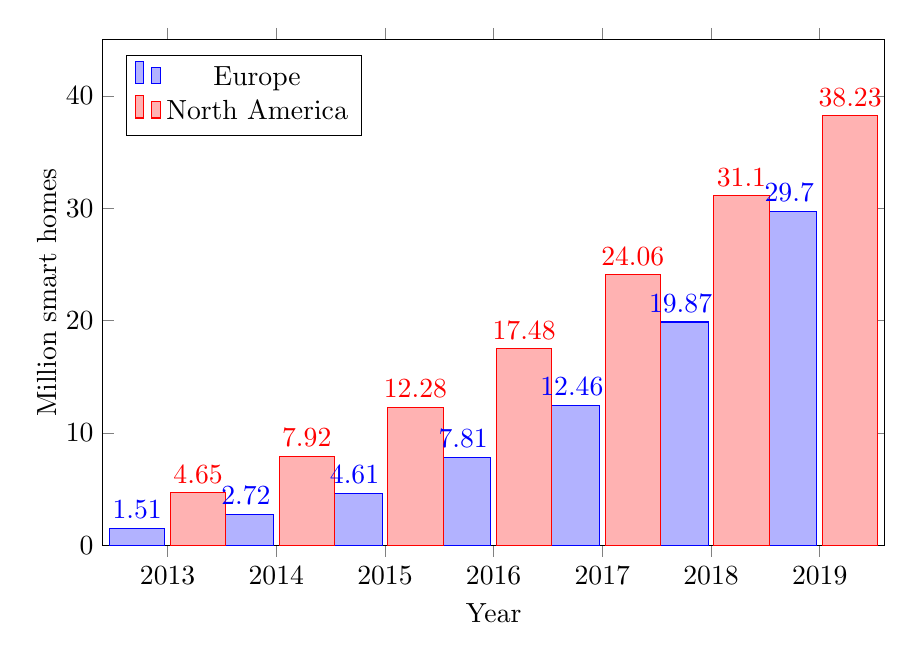
\begin{tikzpicture}
    \begin{axis}[
        height=8cm,
        width=0.95\textwidth,
        xlabel={Year},
        ylabel={Million smart homes},
        yticklabel style={align=right,inner sep=0pt,xshift=-0.3em},
        scaled y ticks = false,
        nodes near coords align={vertical},
        nodes near coords,
        xtick=data,
        symbolic x coords={2013, 2014, 2015, 2016, 2017, 2018, 2019},
        ybar,
        ymax=45,
        ymin=0,
        bar width=20pt,
        legend pos = north west,
        ]
        \addplot coordinates {(2013, 1.51) (2014, 2.72) (2015, 4.61) (2016, 7.81) (2017, 12.46) (2018, 19.87) (2019, 29.70)};        
        \addplot coordinates {(2013, 4.65) (2014, 7.92) (2015, 12.28) (2016, 17.48) (2017, 24.06) (2018, 31.10) (2019, 38.23)};
        \legend{Europe, North America}
        
        %Trend lines:
%        \addplot [ultra thick,orange,line join=round,smooth, nodes near coords = ] coordinates {(2013, 1.51) (2014, 2.72) (2015, 4.61) (2016, 7.81) (2017, 12.46) (2018, 19.87) (2019, 29.70)};
%        \addplot [ultra thick,orange,line join=round,smooth, nodes near coords = ] coordinates {(2013, 4.65) (2014, 7.92) (2015, 12.28) (2016, 17.48) (2017, 24.06) (2018, 31.10) (2019, 38.23)};
%        

    \end{axis}
\end{tikzpicture}}
%     \caption{Smart home. Data from Berg Insight.}
%   \end{figure}
% \end{frame}

% \begin{frame}{Introduction}{Problem}
\begin{frame}{Introduction}{Motivation}
\begin{figure}[h]
\centering
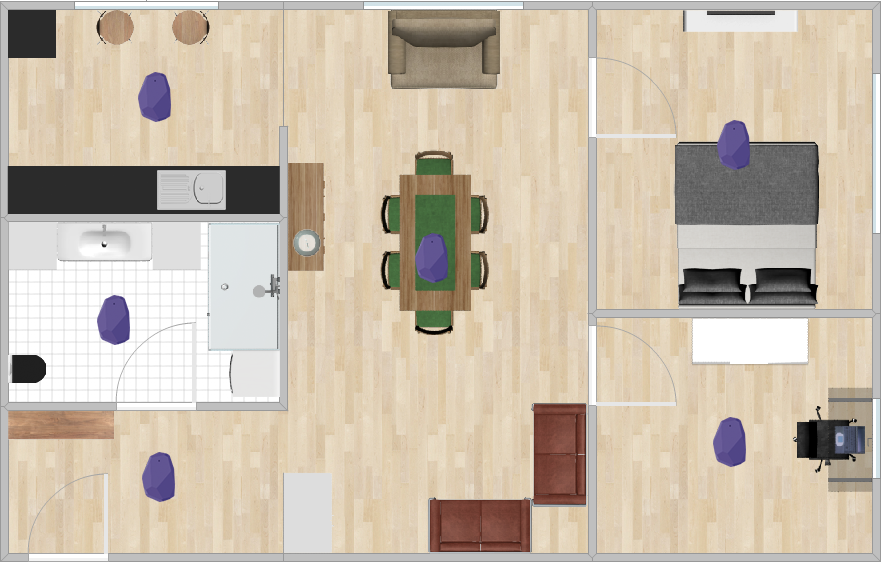
\includegraphics[width=\textwidth]{../images/room-with-beacons}
\caption{Example smart home.}
\end{figure}
\end{frame}

\begin{frame}{Introduction}{Problem}
\begin{block}{Proposed solution}
  \begin{itemize}
    \item Gesture controlled.
    \item Utilizing contextual information.
    \item Virtual positioning of users.
    \item Propose actions when unable to determine one.
  \end{itemize}
\end{block}
\end{frame}

%%% Local Variables:
%%% mode: latex
%%% TeX-master: "../AAUsimpletheme"
%%% End:
